\documentclass{article}

\usepackage{PRIMEarxiv}
\usepackage[utf8]{inputenc}
\usepackage[T1]{fontenc}
\usepackage{hyperref}
\usepackage{url}
\usepackage{booktabs}
\usepackage{amsfonts}
\usepackage{amsmath,amssymb}
\usepackage{nicefrac}
\usepackage{float}
\usepackage{microtype}
\usepackage{fancyhdr}
\usepackage{graphicx}
\usepackage{enumitem}
\usepackage{array}
\usepackage{tabularx}
\usepackage{multirow}
\graphicspath{{./}{../}}

\pagestyle{fancy}
\thispagestyle{empty}
\rhead{\textit{}}
\fancyhead[LO]{Can a Weaker Agent Learn to Win?}

\title{Can a Weaker Agent Learn to Win?\\
Asymmetric Co-Adaptation in Multi-Agent Combat\\
\large Foundations of Artificial Intelligence -- Final Project Report}

\author{
  \textbf{Chirag Agarwalla} \\
  24110093
  \And
  \textbf{Parth Kale} \\
  24110242
  \And
  \textbf{Niraj Kumar} \\
  24110222
  \And
  \textbf{Pallav Biyala} \\
  24110234
}

\begin{document}
\maketitle

\begin{abstract}
Can a mechanically weaker Knight learn to defeat a stronger Boss? We varied Boss health and damage independently over 25 configurations and compared three PPO training schedules across five seeds. Against a fixed heuristic Boss, a Knight trained on that opponent won 86.0\% of games on average at the strongest tested setting. Against paired learned Bosses, simultaneous and alternating learning yielded mean Knight win rates of 71.8\% and 32.7\% at parity, falling to 3.6\% and 1.2\% at the strongest setting. Opponent choice, training order, and variation across seeds limit how broadly these results apply.

\end{abstract}

\keywords{Multi-agent reinforcement learning \and Stochastic games \and PPO \and Asymmetric competition}

\section{Introduction}
Multi-agent reinforcement learning (MARL) studies agents that learn through interaction in a shared environment \cite{busoniu2008comprehensive,zhang2021multi}. In competitive settings, each agent must perform well while responding to an opponent whose policy may also change. This can make learning non-stationary from either agent's perspective \cite{hernandez2020survey}. Competition has produced strong game-playing systems in complex domains \cite{vinyals2019grandmaster} and can generate increasingly sophisticated behavior \cite{bansal2018emergent}; however, performance under a structural capability disadvantage is still an important empirical question.

We ask how much additional health or damage a Boss can have before a trained Knight's mean win rate falls below 50\%. We study this question against a fixed heuristic and against a Boss that learns during training. Varying health and damage independently lets us distinguish the effect of surviving more attacks from the effect of dealing more damage.

\section{Problem Formulation}
\subsection{Game Formalization}
Following the stochastic-game formulation of Shapley and Littman \cite{shapley1953stochastic,littman1994markov}, we model combat as a finite-horizon, two-player game
\begin{equation}
\mathcal{G}= (\mathcal{S},\mathcal{A}_K,\mathcal{A}_B,P,R_K,R_B,\gamma,T),
\end{equation}
where the joint action $(a_K^{(t)},a_B^{(t)})$ induces
$s_{t+1}\sim P(\cdot\mid s_t,a_K^{(t)},a_B^{(t)})$. The episode ends when either agent is defeated, both are defeated in the same transition (draw), or the 300-step limit is reached (timeout/draw). The game engine resolves both agents' selected actions within a shared transition; agents do not take sequential turns.

\subsection{State Space and Capability Asymmetry}
The arena is a $9\times9$ grid. The initial positions are $(4,1)$ for the Knight and $(4,7)$ for the Boss. Each agent receives an agent-relative observation: own/opponent positions (4 values), health and maxima (4), health fractions (2), cooldown features (4), own/opponent combat statistics (12), special windup features (8), and remaining steps (1). A 9-value proposal-state vector adds Knight invulnerability, heal charges, pending-special indicators and origin, dodge cooldown, and dodge/heal enable flags, for 44 input values total. Position and special-origin coordinates are normalized by board dimensions; health, combat statistics, and remaining steps are scaled by 150, 50, and 300, respectively. Action masks are supplied separately and are not part of this vector.

Boss health and damage are independently controlled:
\begin{equation}
H_B(\alpha_H)=\operatorname{round}(150\alpha_H),\qquad
D_B(\alpha_D)=\operatorname{round}(20\alpha_D).
\end{equation}
The Knight has 150 maximum health and basic damage 20. The Boss's basic attack scales with $\alpha_D$; its two special attacks have base damages 50 and 40, also scaled by $\alpha_D$. Thus $\alpha_H$ isolates Boss durability and $\alpha_D$ isolates Boss lethality. At parity $(1,1)$ the Boss has 150 health and 20 basic damage. Special~1 is a directional beam and Special~2 is a radial shockwave. The Boss's basic attack range is one cell; the Knight's basic attack uses Chebyshev distance at most two cells. In this report, ``mechanically weaker'' means that the Knight faces a Boss with $\alpha_H>1$ and/or $\alpha_D>1$, making Boss health and/or damage exceed their parity values; settings below one weaken the corresponding Boss capability, and parity does not imply identical combat kits.

\subsection{Action Spaces}
The Knight action set is
\begin{equation}
\mathcal{A}_K=\{\text{LEFT, RIGHT, UP, DOWN, ATTACK, WAIT, DODGE, HEAL}\},
\end{equation}
and the Boss action set is
\begin{equation}
\mathcal{A}_B=\{\text{LEFT, RIGHT, UP, DOWN, ATTACK, WAIT, SPECIAL\_1, SPECIAL\_2}\}.
\end{equation}
The Knight has three healing charges, each restoring up to 30 health, and a dodge that grants two invincibility frames with a cooldown. Movement, attacks, cooldowns, healing, special-attack telegraphs, collision, and episode termination are resolved by the custom environment.

\subsection{Transition Dynamics and Implemented Rewards}
The proposal initially specified a zero-sum reward based on terminal outcomes and normalized health changes. The completed experiment uses the \texttt{tactical} reward mode: terminal outcomes give $(+1,-1)$ for a Knight win, $(-1,+1)$ for a Boss win, and $(0,0)$ for a draw. Its health-shaping component is based on the potential
\begin{equation}
\Phi_K(s)=w\left(\frac{h_K}{H_K}-\frac{h_B}{H_B}\right),
\qquad
F_K(s,s')=\gamma\Phi_K(s')-\Phi_K(s),
\end{equation}
with $w=0.5$, $\gamma=0.995$, and terminal potential set to zero. The potential-shaping contribution is opposite for the two agents. Draws and timeouts incur an additional common $-0.75$ for both agents.

Tactical event terms for the Knight are: $+0.05$ for a landed attack; $-0.025$ for an attack miss or no-op; $-0.05$ for waiting while an attack is ready; $-0.025$ for waiting when approach is available; $-0.05$ for waiting through an avoidable Special~2; $+0.05$ for dodging damage; $+0.04$ for moving so an incoming Boss attack misses (only when the damage-dodge event did not occur); $-0.025$ for an ineffective dodge, dodge no-op, or heal no-op; and $-0.10$ when Special~1 or Special~2 hits. Knight-only distance shaping rewards closing by $+0.01$ per tile and penalizes retreat by $-0.02$ per tile. The Boss receives the negative of the tactical event delta, but not the Knight-only distance term. These extra terms mean the implemented reward is not strictly zero-sum; in particular, the shared draw penalty and Knight-only distance term are not zero-sum. 



\section{Methodology}
\subsection{Known and Unknown}
The board, actions, combat mechanics, reward definitions, and Boss capability multipliers are specified by the environment; the opposing policy is unknown to a learning agent and must be handled through interaction. Each learned agent receives a vector representation of combat features. PPO action masks are provided separately from this vector: they affect action selection and the action probabilities/log-probabilities used during PPO updates, but are not concatenated to the observation input. The mask rules out currently invalid actions such as moving beyond board boundaries or using a cooling-down action. Attack range is not masked because the opponent may move within the same simultaneous transition.

\subsection{Training Regimes}
We compare three training schedules:
\begin{enumerate}[leftmargin=*,itemsep=1pt]
\item \textbf{Fixed opponent.} Train the Knight using PPO against a scripted heuristic Boss. The Boss follows a fixed rule-based policy and does not learn.
\item \textbf{Simultaneous co-learning.} Initialize the Knight and Boss PPO policies from scratch and update both policies during the same 40,000 environment steps. Each agent has its own actor, critic, optimizer, and rollout data.
\item \textbf{Alternating learning.} During the first 40,000 environment steps, train the Knight against a newly initialized PPO Boss whose policy is frozen and untrained. Then freeze the Knight and train the Boss for 40,000 steps against it. This completed experiment uses one Knight phase followed by one Boss phase; there is no subsequent Knight adaptation phase.
\end{enumerate}
These regimes test a fixed opponent, concurrent adaptation, and a single freeze-and-train response. They do not test repeated alternating rounds.

\subsection{PPO Implementation}
Proximal Policy Optimization (PPO) is a policy-gradient method that uses a clipped objective to discourage excessively large policy updates \cite{schulman2017proximal}. For policy parameters $\theta$, its clipped surrogate objective is
\begin{equation}
L^{\mathrm{CLIP}}(\theta)=
\hat{\mathbb{E}}_t\left[
\min\left(
r_t(\theta)\hat{A}_t,\,
\operatorname{clip}(r_t(\theta),1-\epsilon,1+\epsilon)\hat{A}_t
\right)\right],
\end{equation}
where $r_t(\theta)=\pi_\theta(a_t\mid s_t)/\pi_{\theta_{\mathrm{old}}}(a_t\mid s_t)$, $\hat{A}_t$ is the estimated advantage, and $\epsilon$ is a clipping parameter.

For each rollout, the trainer stores the sampled actions, their masks, rewards, and old log probabilities. It estimates advantages using generalized advantage estimation and updates each active policy on minibatches. Frozen opponents still select actions throughout their phase.
The implementation uses an independent actor--critic PPO system written in the project, rather than Stable-Baselines3. Each policy uses a two-hidden-layer MLP with 128 units per layer. The PPO settings are learning rate $3\times10^{-4}$, discount $\gamma=0.995$, GAE $\lambda=0.95$, clipping range $0.2$, entropy coefficient $0.02$, value coefficient $0.5$, 10 epochs, batch size 64, rollout length 1,024, and maximum gradient norm 0.5. Experiments ran on CPU. Legal-action masks are handled in the actor's distribution and stored separately for probability recomputation; the mask is not part of the actor--critic observation vector.

\section{Experimental Setup}
\subsection{Capability Grid and Training Budget}
We evaluate every pair
\begin{equation}
\alpha_H,\alpha_D\in\{0.5,0.75,1.0,1.25,1.5\},
\end{equation}
for 25 configurations per regime. The five independent training seeds are 0--4, for $25\times3\times5=375$ training runs. Fixed-opponent and simultaneous-learning jobs use 40,000 environment steps each. Alternating jobs use 40,000 steps for the Knight plus 40,000 Boss steps, 80,000 total. The latter therefore has a larger total environment-step budget; regime comparisons are not compute-matched.

Every final Knight checkpoint is evaluated over 500 stochastic games against the heuristic Boss. Simultaneous and alternating checkpoints are also evaluated over 500 games against the final learned Boss paired with that run. For simultaneous learning, that Boss was co-trained with the Knight; for alternating learning, the Boss was trained against the frozen Knight. Neither is a fresh best-response policy. A fresh best-response Boss was not trained in this completed experiment because its training budget was set to zero.

\subsection{Evaluation and Statistical Treatment}
The primary outcome is Knight win rate. Losses, draws, timeouts, and episode length are reported to distinguish defeat from stalemate; a timeout is recorded as a draw, so timeout counts/rates are a subset of draws and must not be added to them. For PPO policies, each seed yields an evaluation win rate over 500 games; reported means and two-sided 95\% Student-$t$ intervals use the five independent training seeds as units. Specifically, the interval is $\bar{x}\pm t_{0.975,4}s/\sqrt{5}$, with sample standard deviation $s$ and $t_{0.975,4}=2.776$. In aggregate tables and win-rate curves, win, loss, draw, and timeout interval endpoints are clipped to $[0,1]$; the seed-variability plot instead draws the un-clipped symmetric intervals. Thus the intervals reflect training-seed variability, not 2,500 independent training runs.

Random and scripted Knight baseline policies are evaluated separately against the heuristic Boss. Their intervals are Wilson binomial confidence intervals from their own 500-game evaluation, not confidence intervals across PPO training seeds. Fixed-opponent training has only heuristic-opponent evaluation; paired learned Boss evaluations exist for simultaneous and alternating runs, with different Boss training procedures as described above.

\subsection{Deviations from the Original Proposal}
\label{sec:deviations}
The proposal used one capability multiplier and included values up to 3. Our computational budget supported a two-dimensional grid up to 1.5 on each axis. We increased evaluation from 100 to 500 games per checkpoint and implemented PPO in PyTorch in place of the proposed Stable-Baselines3 implementation \cite{raffin2021stable}. We also extended the Knight's attack range to two tiles and used tactical reward shaping. We completed one alternating cycle and omitted the proposed fresh best-response evaluation.

\section{Results and Discussion}
\subsection{Random and Scripted Baselines}
The random Knight and scripted Knight are calibration/reference policies, not PPO training seeds. Table~\ref{tab:baselines} reports their separate evaluations against the scripted heuristic Boss at parity and at the strongest tested diagonal setting. At parity, the random Knight wins 8.4\% of games, whereas the scripted Knight wins all 500; at $(1.5,1.5)$, the random Knight wins none and the scripted Knight wins 27.6\%. Equal health and basic damage at parity do not imply a 50\% win rate because the agents have different actions and policies. This gap shows that action selection matters in this environment and that the scripted Knight is a useful non-learning reference. It does not establish that PPO exceeds the scripted policy in all capability settings. The confidence intervals in this table are Wilson intervals from each baseline's 500 evaluation games.

\begin{table}[t]
\centering
\caption{Separate baseline evaluations against the heuristic Boss (500 games per row; Wilson 95\% CI for Knight win rate).}
\label{tab:baselines}
\small
\begin{tabular}{llrrrc}
\toprule
Knight & $(\alpha_H,\alpha_D)$ & Wins & Losses & Draws & Win rate [95\% CI] \\
\midrule
Random & $(1,1)$ & 42 & 456 & 2 & 8.4 [6.3,11.2]\% \\
Scripted & $(1,1)$ & 500 & 0 & 0 & 100 [99.2,100]\% \\
Random & $(1.5,1.5)$ & 0 & 500 & 0 & 0 [0,0.8]\% \\
Scripted & $(1.5,1.5)$ & 138 & 308 & 54 & 27.6 [23.9,31.7]\% \\
\bottomrule
\end{tabular}
\end{table}

\subsection{Capability Heatmaps and Opponent Type}
Figures~\ref{fig:heuristic-heatmap} and \ref{fig:matched-heatmap} show the full 5$\times$5 capability grid. Against the predictable heuristic, the fixed-opponent Knight averages 86.0\% wins at $(1.5,1.5)$ and remains above 50\% throughout the tested grid. Simultaneous and alternating Knights also do well against the heuristic around parity, but their performance degrades more sharply as the Boss becomes stronger. At $(1.5,1.5)$ their heuristic win rates are 32.6\% and 14.6\%, respectively. These results show that training can produce effective policies against this fixed heuristic, but they do not show robustness against an adapting or freshly optimized Boss.

Against the paired learned Boss, performance is substantially lower at higher capabilities. At parity, simultaneous learning averages 71.8\% wins (95\% CI: 30.9--100.0\%) against its co-trained Boss; alternating learning averages 32.7\% (8.0--57.4\%) against the Boss trained against its frozen Knight. At $(1.5,1.5)$ these averages are 3.6\% and 1.2\%. There is also considerable seed variability: parity simultaneous seed win rates range from 17\% to 99\%, while alternating seed rates range from 2\% to 56\%. A high mean from a small sample should not be interpreted as a stable guarantee.

\begin{figure*}[!htbp]
\centering
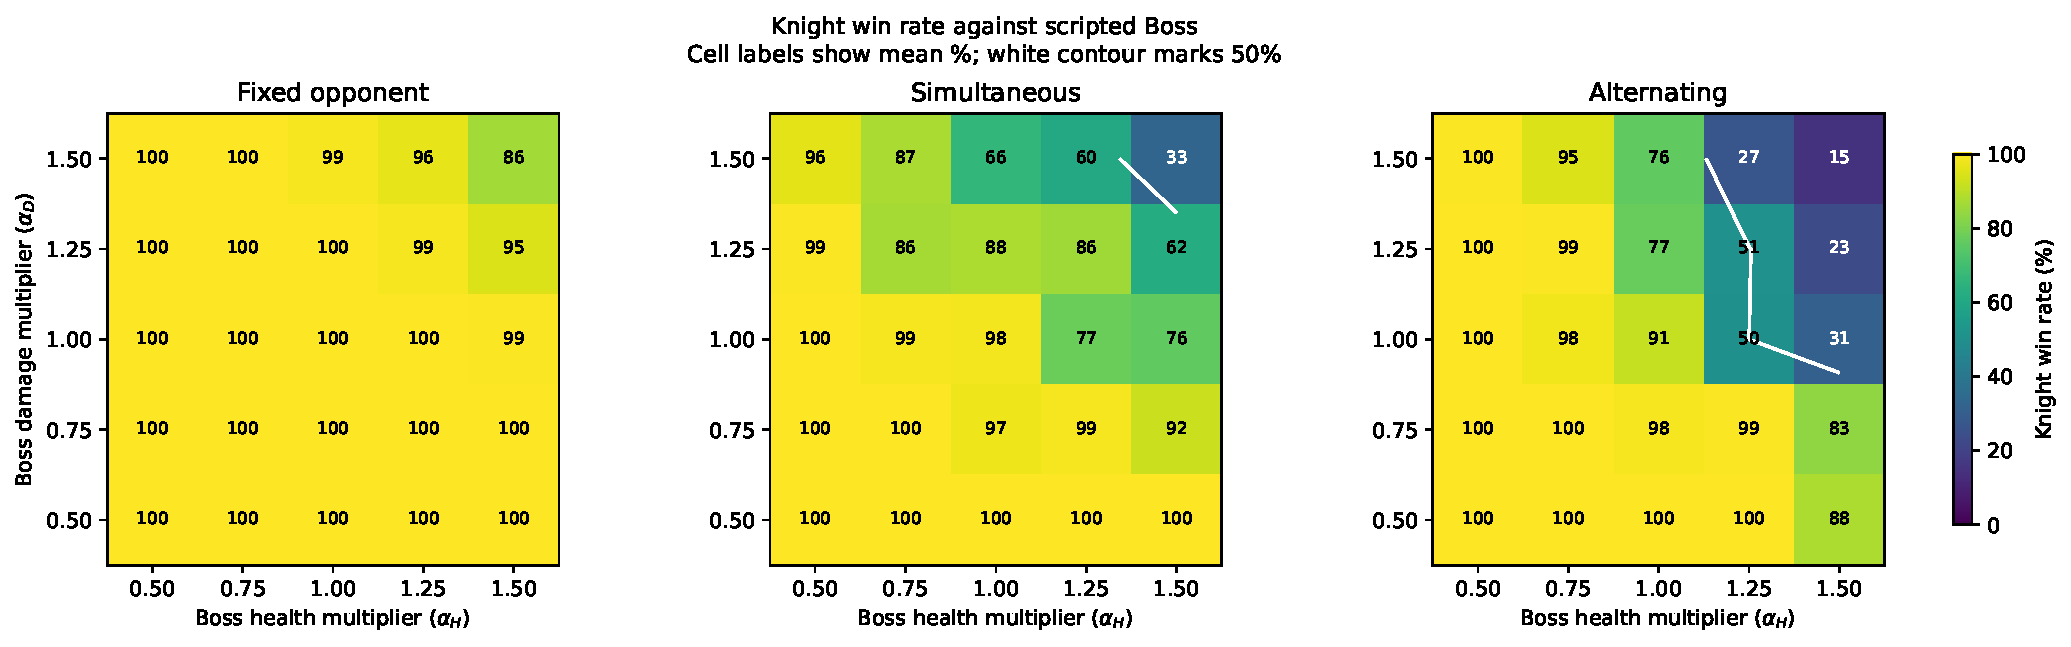
\includegraphics[width=0.96\textwidth]{experiments_action_masked_alpha_fullgrid_v1/analysis/fig_heatmap_heuristic.pdf}
\caption{Knight win rate against the heuristic Boss over the full capability grid. All panels share a 0--100\% color scale; the 50\% contour is shown where applicable.}
\label{fig:heuristic-heatmap}
\end{figure*}

\begin{figure*}[!htbp]
\centering
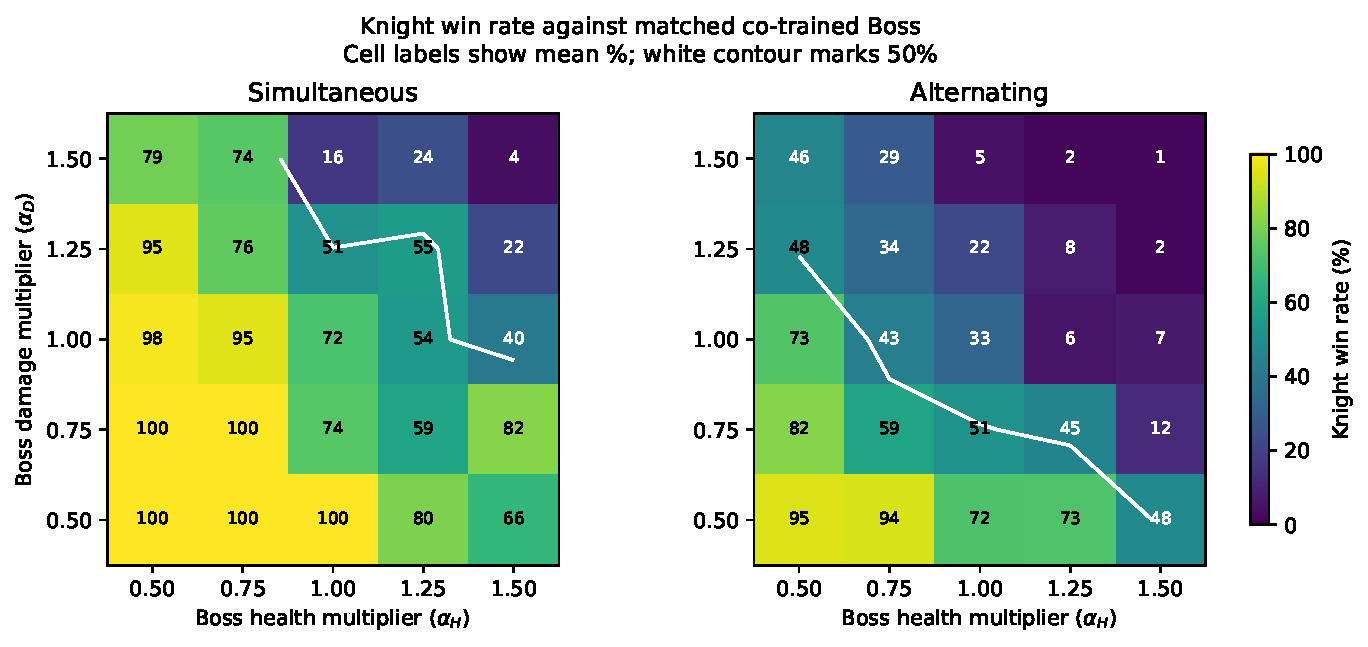
\includegraphics[width=0.83\textwidth]{experiments_action_masked_alpha_fullgrid_v1/analysis/fig_heatmap_matched.pdf}
\caption{Knight win rate against the paired learned Boss: the simultaneous regime's paired co-trained Boss, or the alternating regime's Boss trained against the frozen Knight. Fixed-opponent training has no paired learned Boss. Neither evaluation is a fresh best-response test.}
\label{fig:matched-heatmap}
\end{figure*}

\subsection{Diagonal Comparison}
Figure~\ref{fig:diagonal} compares fixed, simultaneous, and alternating training along $\alpha_H=\alpha_D$. Against the heuristic, the mean Knight win rates at parity are 99.8\% (fixed), 98.1\% (simultaneous), and 91.4\% (alternating). At $(1.5,1.5)$ they are 86.0\%, 32.6\%, and 14.6\%. Against the paired learned Boss, simultaneous versus alternating means are 71.8\% versus 32.7\% at parity, 55.4\% versus 8.0\% at $(1.25,1.25)$, and 3.6\% versus 1.2\% at $(1.5,1.5)$. The simultaneous opponent was co-trained with its Knight; the alternating opponent was trained only after its Knight froze. Fixed-opponent training cannot be ranked on this panel because it has no paired learned Boss. The difference between simultaneous and alternating is suggestive for these settings, but the sample is small, variability is high, and the training budgets differ; it is not evidence of a universally superior schedule.

\begin{figure}[!htbp]
\centering
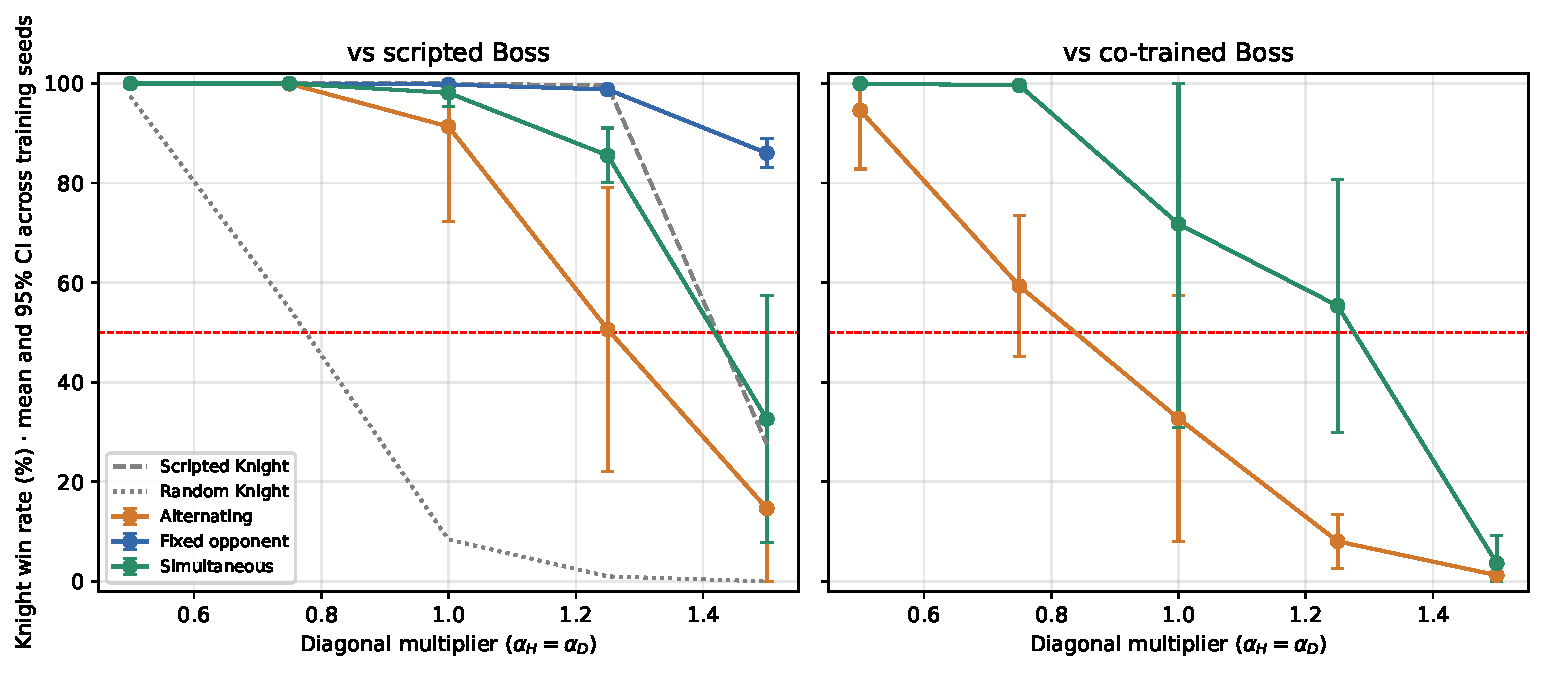
\includegraphics[width=\linewidth]{experiments_action_masked_alpha_fullgrid_v1/analysis/fig_win_vs_alpha.pdf}
\caption{Diagonal Knight win-rate comparison with the heuristic and paired learned Bosses. The simultaneous opponent is co-trained with its Knight; the alternating opponent is trained against the frozen Knight. Markers show five-seed means and error bars show 95\% Student-$t$ intervals.}
\label{fig:diagonal}
\end{figure}

\subsection{Health and Damage Sensitivity}
Figure~\ref{fig:sensitivity} compares durability-only ($\alpha_D=1$) and lethality-only ($\alpha_H=1$) slices. For simultaneous learning against its paired co-trained Boss at multiplier 1.5, the health-only slice yields 40.4\% wins while the damage-only slice yields 16.3\%. For alternating learning against the Boss trained against its frozen Knight at the same endpoint, both slices are poor: 7.0\% for health-only and 4.7\% for damage-only. Against heuristic opponents the ordering varies by regime: for example, at 1.5 the alternating Knight averages 30.6\% on the health-only slice and 75.6\% on the damage-only slice. We therefore find no universal result that Boss health or damage is always the more important constraint. The full grid also reveals interactions that a diagonal-only study would hide. Some curves are non-monotone, so individual slices should be interpreted descriptively rather than as a general law.

\begin{figure}[!htbp]
\centering
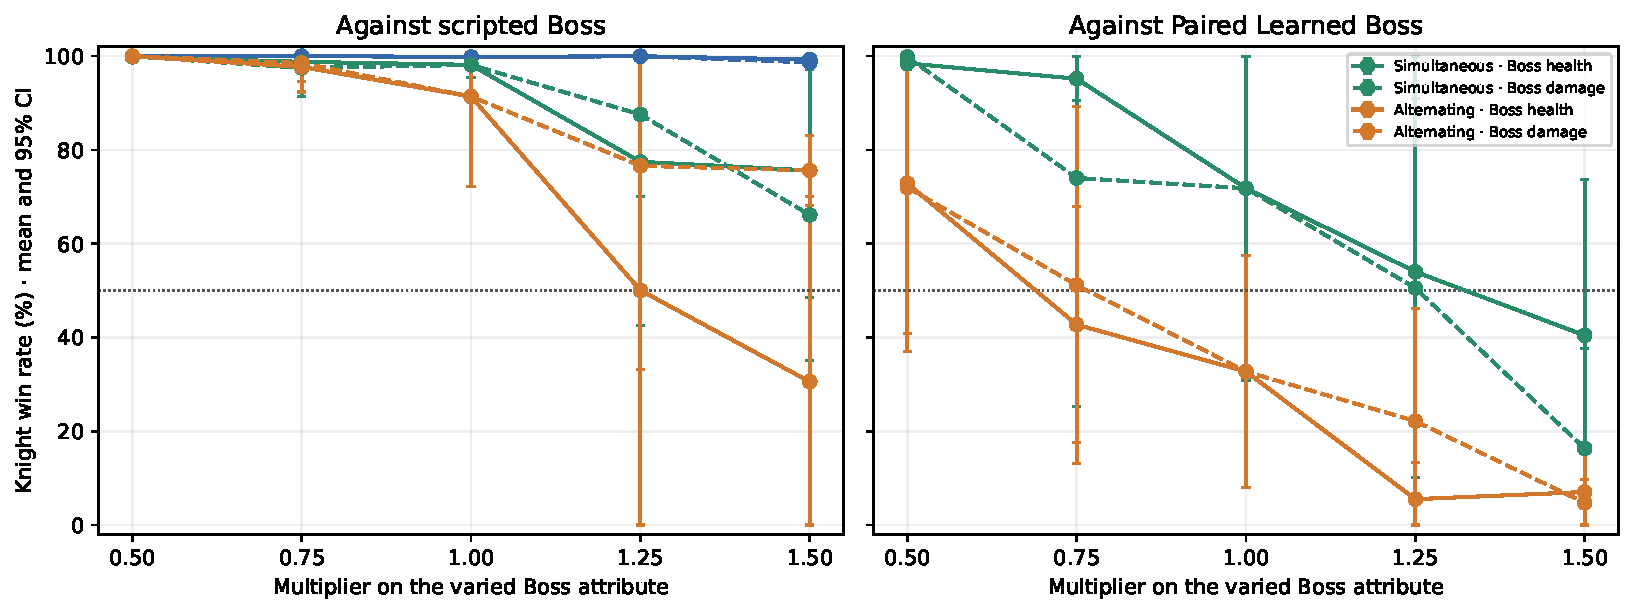
\includegraphics[width=\linewidth]{experiments_action_masked_alpha_fullgrid_v1/analysis/fig_sensitivity.pdf}
\caption{Health-only and damage-only sensitivity slices. The common baseline $(1,1)$ is included on both curves. Error bars are 95\% Student-$t$ intervals across seeds.}
\label{fig:sensitivity}
\end{figure}

\subsection{Seed Variability and Empirical $\alpha^*$}
Figure~\ref{fig:seed-variation} shows seed-level variability along the diagonal against each regime's paired learned Boss. At $(1.25,1.25)$, simultaneous seed rates range from 20\% to 71\%; alternating rates range from 2\% to 13\%. The simultaneous Boss is co-trained with its Knight, while the alternating Boss is trained against its frozen Knight. Wide intervals arise from variation between training runs and reinforce the need for caution with five seeds. The intervals do not remove uncertainty about how these policies would perform under new initializations, opponent policies, or environment variants.

We define $\alpha^*$ as the largest tested value $\alpha\ge1$ on each slice for which the mean Knight win rate is at least 50\%. The three slices are diagonal ($\alpha_H=\alpha_D$), durability ($\alpha_D=1$), and lethality ($\alpha_H=1$). The parity point $(1,1)$ is included in all three analyses. The resulting empirical thresholds are shown in Table~\ref{tab:alpha-star}; they are thresholds on this finite grid, not universal theoretical boundaries. Where the top tested value still qualifies, the threshold is only known to be at least 1.5.

\begin{figure}[!htbp]
\centering
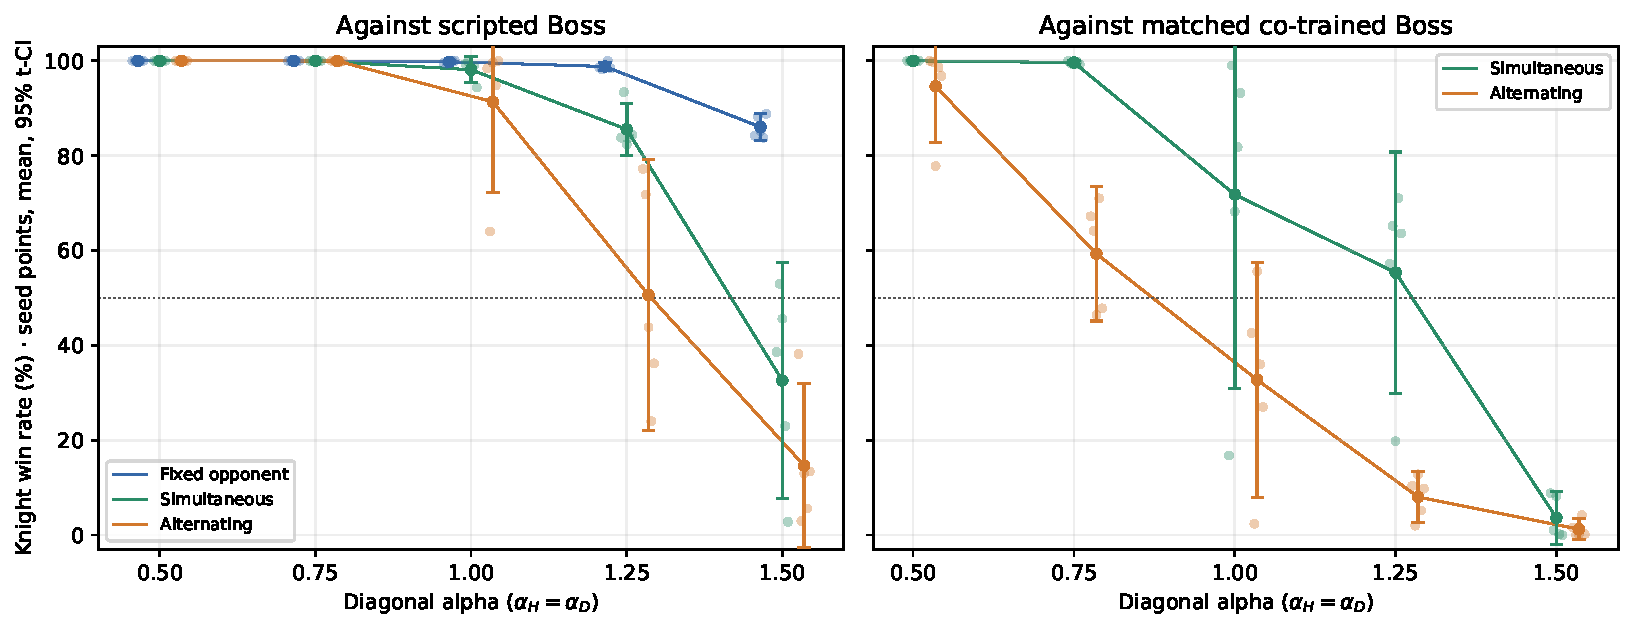
\includegraphics[width=\linewidth]{experiments_action_masked_alpha_fullgrid_v1/analysis/fig_seed_variability.pdf}
\caption{Seed-level diagonal win rates, means, and 95\% Student-$t$ intervals, shown separately for heuristic and paired learned opponents. Simultaneous opponents are co-trained; alternating opponents are trained against their frozen Knights.}
\label{fig:seed-variation}
\end{figure}

\begin{table*}[!htbp]
\centering
\caption{Empirical $\alpha^*$: largest tested multiplier $\ge1$ with mean Knight win rate $\ge50\%$. The baseline is included in all three slices. Values $\ge1.5$ indicate that the threshold is not bounded within the tested range; no qualifying point means none at or above parity qualifies.}
\label{tab:alpha-star}
\small
\begin{tabular}{llccc}
\toprule
Training regime & Opponent & Diagonal & Durability & Lethality \\
\midrule
Fixed & Heuristic & $\ge1.5$ & $\ge1.5$ & $\ge1.5$ \\
Simultaneous & Heuristic & 1.25 & $\ge1.5$ & $\ge1.5$ \\
Alternating & Heuristic & 1.25 & 1.25 & $\ge1.5$ \\
Simultaneous & Paired learned & 1.25 & 1.25 & 1.25 \\
Alternating & Paired learned & None & None & None \\
\bottomrule
\end{tabular}
\end{table*}

\section{Limitations}
At parity, the simultaneously trained Knight won 71.8\% of games on average against its paired Boss, but individual training seeds ranged from 17\% to 99\%. The 500 games per checkpoint help estimate how often that particular policy wins. With only five independently trained policies per setting, the mean remains sensitive to which seeds were sampled. We evaluated final checkpoints, so the results also leave open how quickly each regime learned or whether performance had stabilized.

Training order and budget both affect the comparison. Fixed-opponent and simultaneous learning each used 40,000 environment steps. Alternating learning used 80,000 steps in a single cycle: 40,000 for the Knight, then 40,000 for the Boss against the frozen Knight. The Knight had no opportunity to respond to that final Boss. Isolating the effect of training order would require matched budgets and repeated response phases.

The heuristic Boss follows predictable rules. Against learned opponents, each Knight faced the Boss from its own run: a co-trained Boss in simultaneous learning and a Boss trained against the frozen Knight in alternating learning. Performance against a fresh best-response Boss remains untested. The findings also depend on this game's simultaneous actions, attack ranges, action masks, and shaped tactical reward. We did not systematically vary the reward terms or PPO hyperparameters to measure their individual effects.

Available time and compute limited the sweep to five values per axis between 0.5 and 1.5. The 25 health--damage combinations already required 375 training runs, whose recorded durations sum to about 6 hours 11 minutes. Adding even one value to both axes would increase the grid to 36 combinations and require 165 additional runs at the same three regimes and five seeds. The empirical $\alpha^*$ in Table~\ref{tab:alpha-star} therefore describes the tested grid. Where the mean win rate still reaches 50\% at 1.5, the upper threshold remains open.

\section{Contributions}

\begin{table}[H]
\centering
\caption{Original assigned responsibilities and team-reported fulfillment status.}
\label{tab:contributions}
\small
\begin{tabularx}{\textwidth}{@{}p{0.20\textwidth}X p{0.24\textwidth}@{}}
\toprule
Member & Assigned responsibility in the proposal & Fulfillment status \\
\midrule
Pallav Biyala & Environment design and documentation: define game mechanics, finalize mathematical formulation, maintain proposal/report, and coordinate integration. & Completed (team-confirmed) \\
Chirag Agarwalla & Environment implementation: build the combat simulation and implement movement, attacks, health, cooldowns, healing, and termination. & Completed (team-confirmed) \\
Parth Kale & PPO implementation: implement PPO for both agents, define observations and rewards, and enable multi-agent training. & Completed (team-confirmed) \\
Niraj Kumar & Training experiments and evaluation: implement regimes, run capability experiments, calculate win rates, and generate plots. & Completed (team-confirmed) \\
\bottomrule
\end{tabularx}
\end{table}

Table~\ref{tab:contributions} records the team's assessment of each assigned task.

\section{Conclusion}
We asked whether a mechanically weaker Knight can learn to defeat a stronger Boss that may also learn. In this environment, the answer is conditionally yes. The Knight trained against a fixed heuristic performs strongly over the tested grid, while evaluation against the paired learned Boss becomes difficult as Boss capabilities rise. At parity, simultaneous learning has a 71.8\% mean win rate against its paired co-trained Boss, but the 95\% interval across five seeds is wide; the one-switch alternating regime averages 32.7\% against its Boss trained against the frozen Knight. At the strongest diagonal setting, both win rates are near zero.

The results support the claim that learning can produce an underdog policy that wins under some conditions. They do not show that a Knight can reliably beat an arbitrary or best-response learning Boss. Capability effects depend on opponent and training regime, and the five-seed variability and unequal budgets limit causal comparisons. A stronger follow-up would equalize training budgets, use repeated alternating rounds, increase independent seeds, and evaluate against fresh best-response Bosses.

\section*{Code Availability}

The source code for the custom combat environment, PPO implementation, training procedures, and evaluation scripts is available at:

\url{https://github.com/Pallav-Biyala/FAI-Project-Knight-vs-Boss-MARL}

\begin{thebibliography}{99}

\bibitem{busoniu2008comprehensive}
L.~Bu{\c{s}}oniu, R.~Babu{\v{s}}ka, and B.~De Schutter,
\textquotedblleft A comprehensive survey of multiagent reinforcement learning,\textquotedblright
\emph{IEEE Transactions on Systems, Man, and Cybernetics, Part C (Applications and Reviews)}, vol.~38, no.~2, pp.~156--172, 2008.

\bibitem{zhang2021multi}
K.~Zhang, Z.~Yang, and T.~Ba{\c{s}}ar,
\textquotedblleft Multi-agent reinforcement learning: A selective overview of theories and algorithms,\textquotedblright
in \emph{Handbook of Reinforcement Learning and Control}, Springer, 2021, pp.~321--384.

\bibitem{shapley1953stochastic}
L.~S. Shapley,
\textquotedblleft Stochastic games,\textquotedblright
\emph{Proceedings of the National Academy of Sciences}, vol.~39, no.~10, pp.~1095--1100, 1953.

\bibitem{littman1994markov}
M.~L. Littman,
\textquotedblleft Markov games as a framework for multi-agent reinforcement learning,\textquotedblright
in \emph{Proceedings of the 11th International Conference on Machine Learning (ICML)}, 1994, pp.~157--163.

\bibitem{schulman2017proximal}
J.~Schulman, F.~Wolski, P.~Dhariwal, A.~Radford, and O.~Klimov,
\textquotedblleft Proximal policy optimization algorithms,\textquotedblright
\emph{arXiv preprint arXiv:1707.06347}, 2017.

\bibitem{hernandez2020survey}
P.~Hernandez-Leal, B.~Kartal, and M.~E. Taylor,
\textquotedblleft A survey and critique of multiagent deep reinforcement learning,\textquotedblright
\emph{Autonomous Agents and Multi-Agent Systems}, vol.~33, no.~6, pp.~750--797, 2019.

\bibitem{bansal2018emergent}
T.~Bansal, J.~Pachocki, S.~Sidor, I.~Sutskever, and O.~Mordatch,
\textquotedblleft Emergent complexity via multi-agent competition,\textquotedblright
in \emph{International Conference on Learning Representations (ICLR)}, 2018.

\bibitem{vinyals2019grandmaster}
O.~Vinyals et al.,
\textquotedblleft Grandmaster level in StarCraft II using multi-agent reinforcement learning,\textquotedblright
\emph{Nature}, vol.~575, pp.~350--354, 2019.

\bibitem{raffin2021stable}
A.~Raffin, A.~Hill, A.~Gleave, A.~Kanervisto, M.~Ernestus, and N.~Dormann,
\textquotedblleft Stable-Baselines3: Reliable reinforcement learning implementations,\textquotedblright
\emph{Journal of Machine Learning Research}, vol.~22, no.~268, pp.~1--8, 2021.

\end{thebibliography}

\end{document}
